\section{Introduction}
In this section, we can talk about 
\begin{itemize}
    \item The trend of ML  in CPS and the need of safety AI.
    \item The safe fail technique, and the need to determine whether to reject predict.
\end{itemize}



\subsection{Background: Prediction with Uncertainty}
For classification problems,  the output of ML models is usually interpreted as model confidence in that prediction. For example,  output obtained at the end of the softmax layers of standard deep learning are often interpreted the predictive probabilities. If the obtained ``confidence'' level is very low, the models could select a reject option. A support vector machine (SVM) like classifier for classification with a reject option is proposed in~\cite{bartlett2008} for binary classification problems. For ensemble classifiers, the votes of base classifiers~\cite{varshney2013practical} will be used to determine whether to reject a prediction.  

The implicit assumption shared by classifiers is that ML models are most uncertain near the boundary between the different classes  and the distance from the decision boundary is inversely related to the confidence that the instance belong to that class. This is reasonable  to some extents because the decision boundaries learned by these models are usually located where a lot training samples belong to different classes overlap.   However, for feature space $\mathcal X$ that  contain few or no training samples at all,  then the learned the decision boundary may be completely based on an inductive bias, thereby containing much epistemic uncertainty~\cite{Attenberg:2015}. It is possible that an input instance that far from any training samples would be classified as some class  with very high probability~\cite{gal2016dropout}. 

Prediction uncertainty can also be obtained by Bayesian inference.  Bayesian probability theory provides a mathematically grounded tool to model the prediction uncertainty.   Gaussian process (GP)~\cite{seeger2004gaussian} is a  well known   probabilistic model and assumes that $p(f(\mathbf x_1), \ldots, f(\mathbf x_N ))$ is jointly Gaussian, with some mean $\mu(\mathbf x)$ and covariance $\Sigma(\mathbf x)$.  Given training samples $(\mathbf X,\mathbf y)$ and unobserved instance $\mathbf x_*$, the output $\mathbf f_*$ is also conditional Gaussian $p(\mathbf f_*|x_*,\mathbf X,\mathbf y)=\mathcal N(\mu_*,\sigma_*)$ where the standard deviation can be interpreted as the prediction confidence. GP is  computational intensive and has complexity $O(N^3)$, where N is the number of data.  Bayesian methods can also be applied to neural networks (NNs). Infinitely wide single hidden layer NNs with distributions placed over their weights converge to Gaussian processes~\cite{neal2012bayesian}. Variational inference~\cite{paisley2012variational,kingma2013auto} can be used to obtain  approximations for finite Bayesian neural networks. The  dropout  techniques in NNs can also be interpreted as a Bayesian approximation of  Gaussian process~\cite{gal2016dropout}. With all the good properties of Bayesian learning,  there are some  controversial aspects: 1) is its reliance on priors and  2) it is  computationally intensive.

The conformal prediction framework~\cite{Vovk:2005,vovk2009line} uses past experience to determine precise levels  of confidence in new predictions. Given a certain error probability $\epsilon$ requirement, it forms a prediction interval $[\overline{f(\mathbf x)},\underline{{f(\mathbf x)}}]$ for regression or a  prediction label set $\{\mbox{Label 1},\mbox{Label 2},\ldots \}$ for classification  so that the interval/set contains the actual prediction with probability $1-\epsilon$. However, its theoretically accuracy guarantee depends on the assumption that all the data are independent and identically distributed (in fact, i.i.d. assumption replaced by the weaker assumption of ``exchangeability'').  Besides, for regression problems, it tends to  produce prediction bands  whose width is roughly constant over the whole feature space~\cite{lei2018distribution}.





















\subsection{Motivation}
Data-driven  models are trained by ML learning algorithms using a subset of possible scenarios that could be encountered operationally.   Thus,  the models produced by ML algorithms  can only be as good as the examples that have learned.  However, the training set is usually incomplete and there is no guarantee that it is even representative of the space of possible inputs~\cite{ISO16}.  Previous study~\cite{weiss1995learning} has demonstrated that  feature space that lack of data generally have a much higher error rate.    

For example, Figure~\ref{fig:toy1} shows the decision boundary learned by a SVM classifier to predict the whether a wall-following  robot is turning right sharply.  The value in the contour map represents the probability learned by the classifier that the instance belong to class ``Sharp-Right-Turn''.  As we can observe, the training samples is not  representative of testing samples at all. However, the classifier still has relative high confidence in some regions where it has not well learned but lots of many testing samples locates. As a result, a lot of testing samples that belong to other classes are misclassified as ``Sharp-Right-Turn'', and accuracy for testing samples decreases to $66\%$ while the accuracy for training samples is almost $100\%$. In practice, safety-critical scenarios like traffic accidents are very rare and ML algorithms usually do not receive enough such training samples.


\begin{figure}[t]
\centering
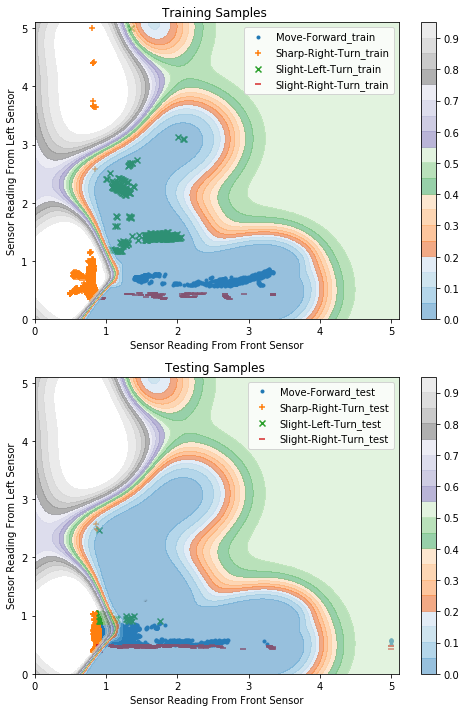
\includegraphics[width=0.45\textwidth]{FIG/toy1.png}
\caption{Wall-following navigation task with mobile robot SCITOS-G5 based on sensor readings from the front and left sensor~\cite{Dua:2017}.}
\label{fig:toy1}
\end{figure}


Therefore, it is very important to identify the feature space that the model is not well trained from that it does not receive enough training samples.

 % so that safety-critical systems with ML component could  REJECT OR GET MORE TRAINING SAMPLES

\noindent\textbf{Desired Characteristics}